\documentclass{beamer}
\usetheme{CMU}

\usepackage{pgf,pgfarrows,pgfnodes,pgfautomata,pgfheaps,pgfshade}
\usepackage{amsmath,amssymb}
\usepackage[utf8]{inputenc}
\usepackage{colortbl}
\usepackage[english]{babel}
\usepackage{booktabs}
\usepackage{slpython}
\usepackage{underscore}

\author{Luís Pedro Coelho}
\institute{Programming for Scientists}

\graphicspath{{figures/}{figures/generated/}{images/}}

\newcommand*{\code}[1]{\textsl{#1}}


\title{Numerical Representations}
\begin{document}
\frame{\maketitle}

\begin{frame}[fragile]
\frametitle{How Are Numbers Represented}

It's all 0s \& 1s. How do you represent 123?

\end{frame}

\begin{frame}[fragile]
\frametitle{Binary Notation}

$(b_4b_3b_2b_1b_0)_2 = b_4 2^4 + b_3 2^3 + b_2 2^2 + b_1 2^1 + b_0 2^0 = 16b_4 + 8b_3 + 4b_2 + 2 b_1 + b_0$

\end{frame}

\begin{frame}[fragile]
\frametitle{Common Number Sizes}

\begin{itemize}
\item Byte: 8 bits, 0 to 255 ($2^8-1$).
\item Short: 16 bits, 0 to 65535 ($2^{16}-1$).
\item 32-bit int: 32 bits, 0 to 4294967295 ($2^{32}-1$).
\item 64-bit int: 64 bits, 0 to 18446744073709551615 ($2^{64}-1$).
\end{itemize}
\end{frame}

\begin{frame}[fragile]
\frametitle{Bit-wise operations}

\begin{enumerate}
\item NOT(A): true if A is \alert{not} true (\lstinline{~A})
\item AND(A,B): true if A is true and B is true (\lstinline{A \& B})
\item OR(A,B): true if either A or B are true (\lstinline{A | B})
\item XOR(A,B): true if one is true and the other is false \lstinline{A \^ B}
\end{enumerate}

\note{
    Two ways to view a number: as a number or as a collection of bits.
}
\end{frame}

\begin{frame}[fragile]
\begin{python}
def fact(N):
     if N == 0: return 1
     return N * fact(N-1)

print  fact(100)
\end{python}

Prints out

933262154439441526816992388562667004907159682643816214\\
685929638952175999932299156089414639761565182862536979\\
20827223758251185210916864000000000000000000000000L

\end{frame}

\begin{frame}[fragile]

What about negative numbers?

\end{frame}

\begin{frame}[fragile]

\begin{itemize}
\item Sign bit
\item Ones' complement
\item Twos' complement,
\end{itemize}
\end{frame}

\begin{frame}[fragile]
\frametitle{Sign Bit}

$(s b_4 b_3 b_2 b_1 b_0)_2 = (-1)^s \left(b_4 2^4 + b_3 2^3 + b_2 2^2 + b_1 2^1 + b_0 2^0 = 16b_4 + 8b_3 + 4b_2 + 2 b_1 + b_0\right)$

\end{frame}

\begin{frame}[fragile]
\frametitle{One's Complement}

If $(b_k b_{k-1}\cdots b_1 b_0)_2$ is some number $n$, then we represent $-n$ by\\
$(\tilde{}b_k \tilde{}b_{k-1}\cdots \tilde b_1 \tilde{} b_0)_2$ is some number $n$, then we represent $-n$ by

\pause

$(00000011)_2$ is $\phantom{-}3$\\
$(11111100)_2$ is $-3$

\bigskip

$(00001111)_2$ is $\phantom{-}31$\\
$(11110000)_2$ is $-31$

\bigskip

$(00000000)_2$ is $\phantom{-}0$\\
$(11111111)_2$ is $-0$


\pause

Ones' complement is not actually used in any modern machine.

\end{frame}

\begin{frame}[fragile]
\frametitle{Twos' Complement}

\centering
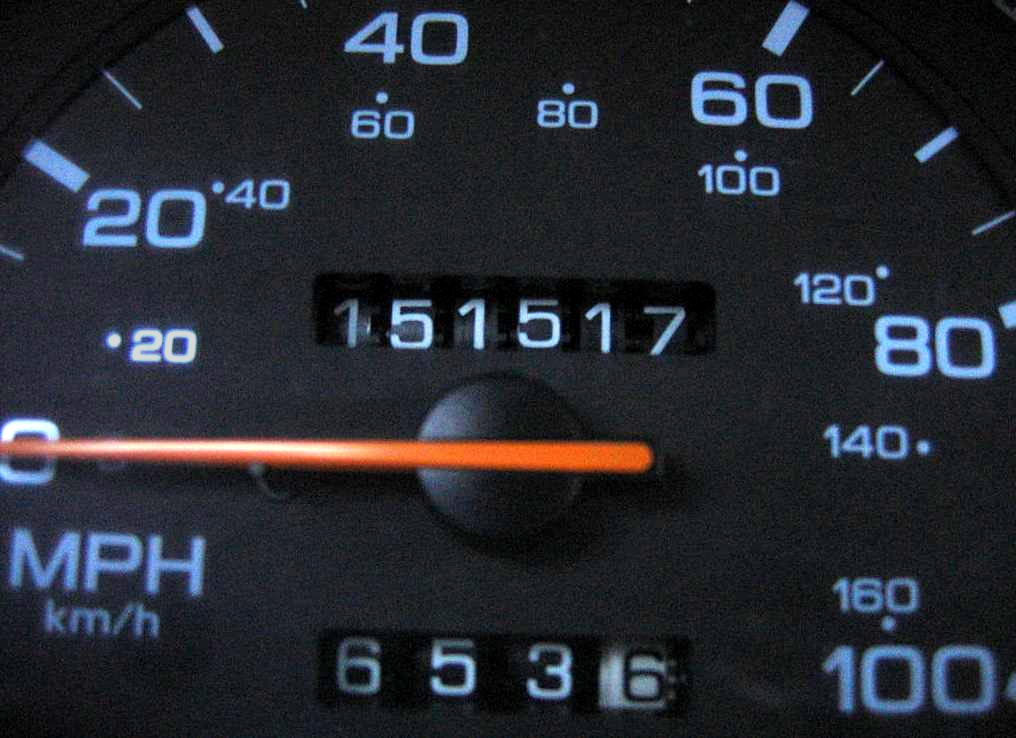
\includegraphics{Odometer2.jpg}

\begin{flushright}
Image from Wikipedia\\
Metaphor from Steve Heller
\end{flushright}
\end{frame}

\begin{frame}[fragile]
\frametitle{Twos' Complement}

$(11111111)_2$ is $-1$

$(11111110)_2$ is $-2$

$(11111101)_2$ is $-3$

\note{
    Show addition/subtraction of 2s complement.

    Note that we do have a sign bit.
}
\end{frame}

\begin{frame}[fragile]
\frametitle{Ranges}

\begin{itemize}
\item 8 bits: $-128$ to $127$.
\item 16 bits: $-32768$ to $32767$.
\item 32 bits: $-2147483648$ to $2147483647$.
\item 64 bits: $-9223372036854775808$ to $9223372036854775807$.
\end{itemize}
\end{frame}

\begin{frame}[fragile]
\frametitle{Fractional Numbers}

What about fractional numbers?

\begin{itemize}
\item Fixed point
\item Floating point
\end{itemize}

\end{frame}

\begin{frame}[fragile]
\frametitle{Fixed Point}

Given a fixed base $B$, then an integer $n$ really represents the number $n * 2^B$.

\note{
    Mention how this is used for money.
}

\end{frame}

\begin{frame}[fragile]
\frametitle{Floating Point}
<+content+>
\end{frame}<++>
\end{document}
